% --------------------------------------------------------------
% This is all preamble stuff that you don't have to worry about.
% Head down to where it says "Start here"
% --------------------------------------------------------------
 
\documentclass[12pt]{article}
\usepackage{textcomp}
\usepackage[margin=1in]{geometry} 
\usepackage{amsmath,amsthm,amssymb}
\usepackage[margin=1in]{geometry} 
\usepackage{amsmath,amsthm,amssymb}
\usepackage[spanish]{babel} %Castellanización
\usepackage[T1]{fontenc} %escribe lo del teclado
\usepackage[utf8]{inputenc} %Reconoce algunos símbolos
\usepackage{lmodern} %optimiza algunas fuentes
\usepackage{graphicx}
\graphicspath{ {images/} }
\usepackage{hyperref} % Uso de links
 
\newcommand{\N}{\mathbb{N}}
\newcommand{\Z}{\mathbb{Z}}
 
\newenvironment{theorem}[2][Theorem]{\begin{trivlist}
\item[\hskip \labelsep {\bfseries #1}\hskip \labelsep {\bfseries #2.}]}{\end{trivlist}}
\newenvironment{lemma}[2][Lemma]{\begin{trivlist}
\item[\hskip \labelsep {\bfseries #1}\hskip \labelsep {\bfseries #2.}]}{\end{trivlist}}
\newenvironment{exercise}[2][Exercise]{\begin{trivlist}
\item[\hskip \labelsep {\bfseries #1}\hskip \labelsep {\bfseries #2.}]}{\end{trivlist}}
\newenvironment{problem}[2][Problem]{\begin{trivlist}
\item[\hskip \labelsep {\bfseries #1}\hskip \labelsep {\bfseries #2.}]}{\end{trivlist}}
\newenvironment{question}[2][Question]{\begin{trivlist}
\item[\hskip \labelsep {\bfseries #1}\hskip \labelsep {\bfseries #2.}]}{\end{trivlist}}
\newenvironment{corollary}[2][Corollary]{\begin{trivlist}
\item[\hskip \labelsep {\bfseries #1}\hskip \labelsep {\bfseries #2.}]}{\end{trivlist}}

\newenvironment{solution}{\begin{proof}[Solution]}{\end{proof}}
 \usepackage{multicol}
%AAqui inicia la parte importante del documento


\begin{document}

\twocolumn[

\begin{@twocolumnfalse}
\title{\Huge  Examen correspondiente al área de geometría}
\author{Elaborado por el CUEP \\ 10 preguntas - 17 minutos}
\date{}
\maketitle
\end{@twocolumnfalse}
]

\begin{figure}[h]
\centering
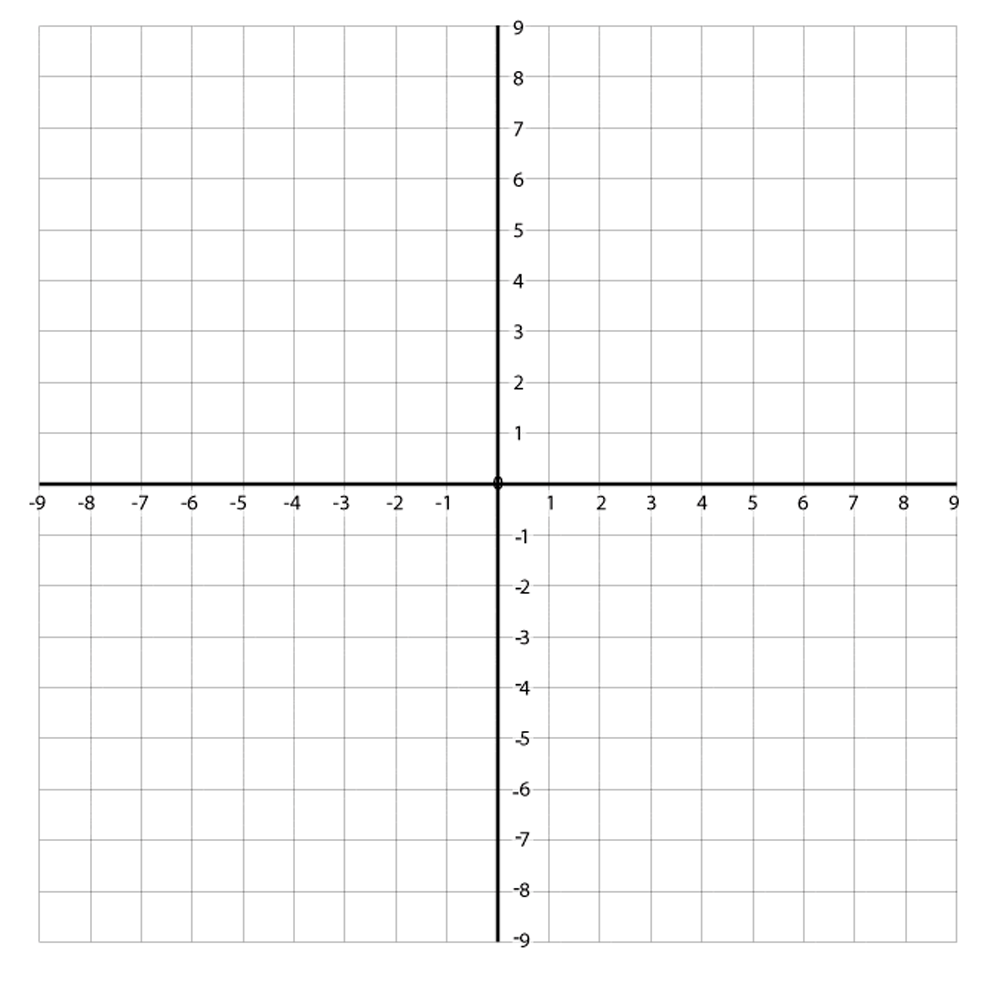
\includegraphics[scale=0.13]{imagenes/PlanoCartesiano.png} 
\caption{}
\label{etiqueta}
\end{figure}
\begin{enumerate} %Lista enume\mathbf{i}rada

\item  Observando la figura 1 hallar la distancia entre los puntos $(0,-2) \ (4,-6)$.

\begin{enumerate}
    \item $8{\sqrt 20}$
    \item ${\sqrt 32}$  
    \item $ 7.623623 $
    \item $ 16$ 
    \item $4{\sqrt 5}$
    \end{enumerate}
    
\item  Observando la figura 1 hallar la distancia entre los puntos $(-2,2) \ (8,10)$.

\begin{enumerate}
    \item $ \sqrt 164$
    \item $ \sqrt 180 $  
    \item $ 5 \sqrt 10 $
    \item $ 10 $ 
    \item $ 5 $
    \end{enumerate}

\item  Tomando la fig.1 ¿Cuál es el área del triángulo formado en los puntos \\ $(1,1) \ (5,1) \ (1,4)$?
\begin{enumerate}
    \item $ 12 \ u^2 $
    \item $ 6 \ u^2 $  
    \item $ 3 \sqrt 3 \ u^2 $
    \item  No se puede determinar  
    \item $ 20 \ u^2 $
    \end{enumerate}

\begin{figure}[h]
\centering
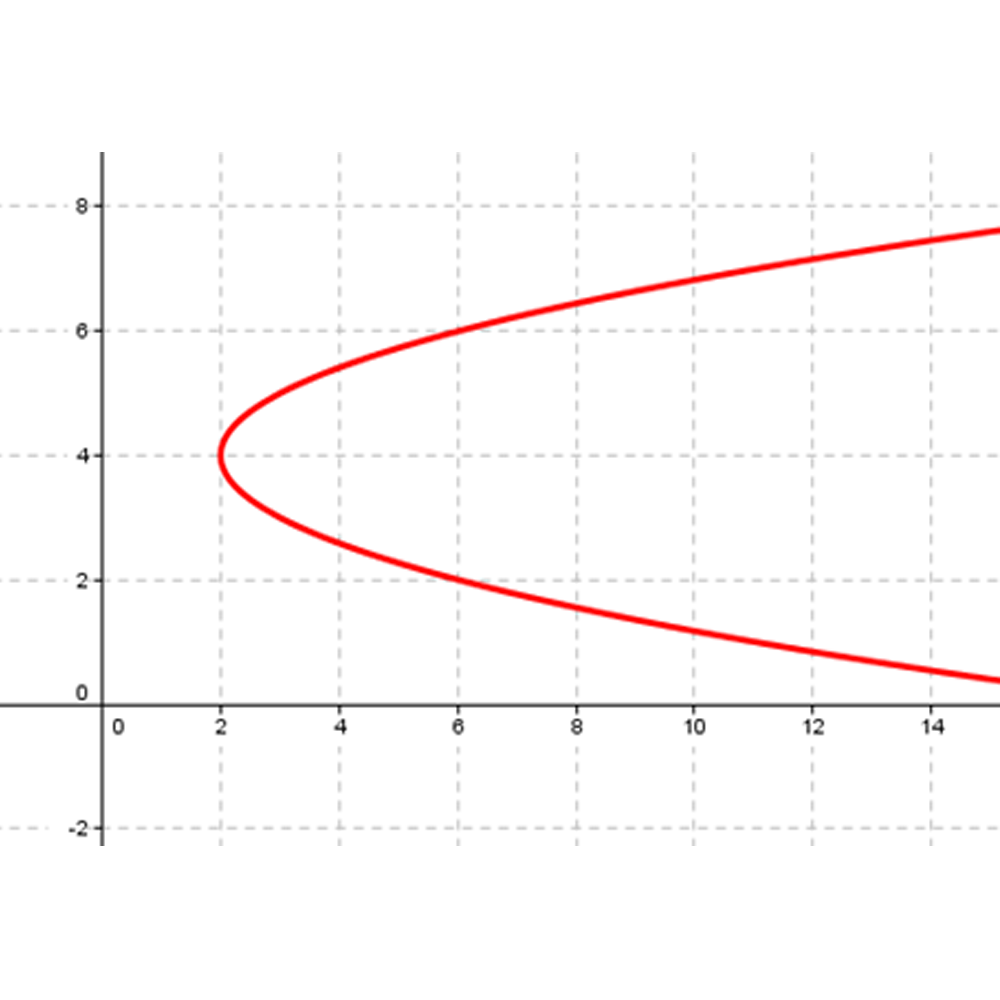
\includegraphics[scale=0.15]{imagenes/parabola1.png} 
\caption{}
\label{etiqueta1}
\end{figure}

\item  ¿Cuál de las siguientes ecuaciones representa la parábola de la figura 2?
\begin{enumerate}
    \item $ (y-4)^2 \ = 4p \ (x-2) $
    \item $ (y-2)^2 \ = 4p \ (x+4) $  
    \item $ (y+4)^2 \ = 4p \ (x+2) $
    \item $ (x-4)^2 \ = 4p \ (y-2) $  
    \item $ (x-2)^2 \ = 4p \ (x-4) $
    \end{enumerate}

\begin{figure}[h]
\centering
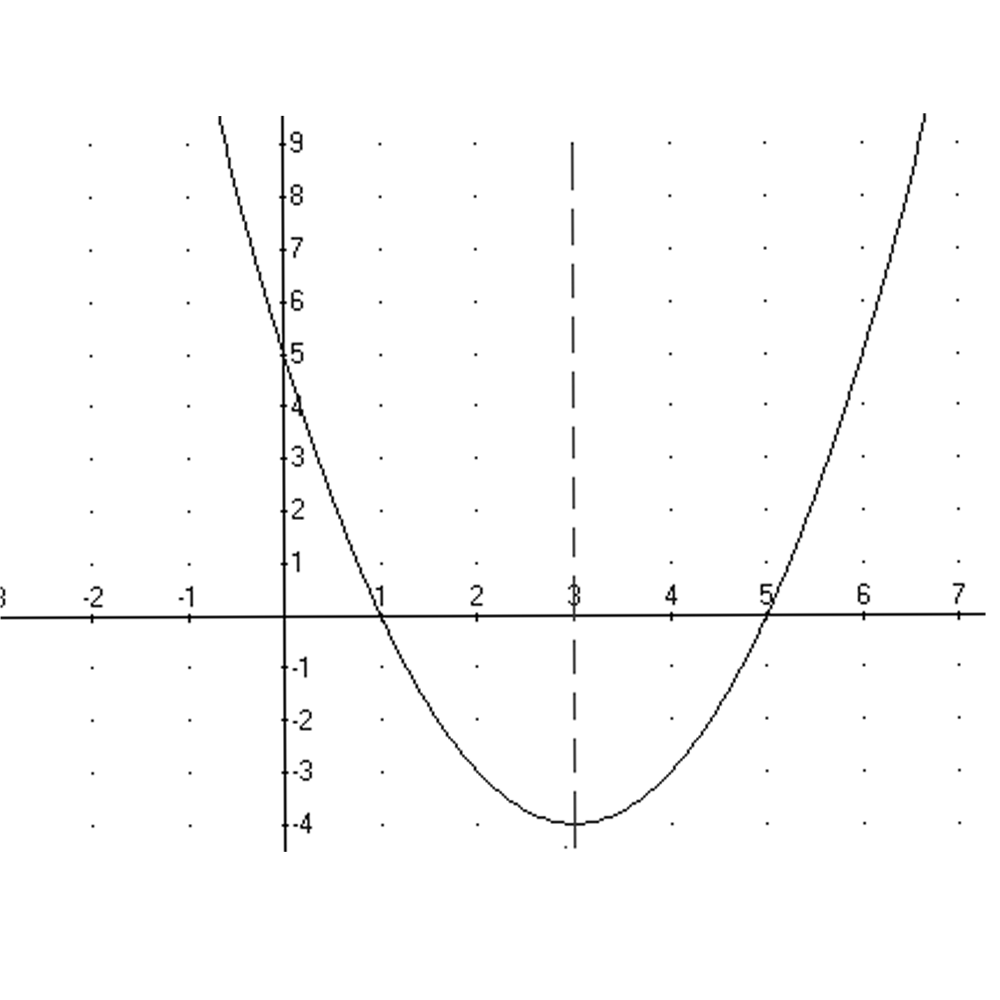
\includegraphics[scale=0.15]{imagenes/parabola2.png} 
\caption{}
\label{etiqueta2}
\end{figure}

\item  ¿Cuál de las siguientes ecuaciones representa la parábola de la figura 3? \\
\begin{enumerate}
    \item $ (y+3)^2 \ = 4p \ (x-4) $
    \item $ (y-3)^2 \ = 4p \ (x-4) $  
    \item $ (y+4)^2 \ = 4p \ (x+3) $
    \item $ (x-3)^2 \ = 4p \ (y+4) $  
    \item $ (x+3)^2 \ = 4p \ (x-4) $
    \end{enumerate}
    
\begin{figure}[h]
\centering
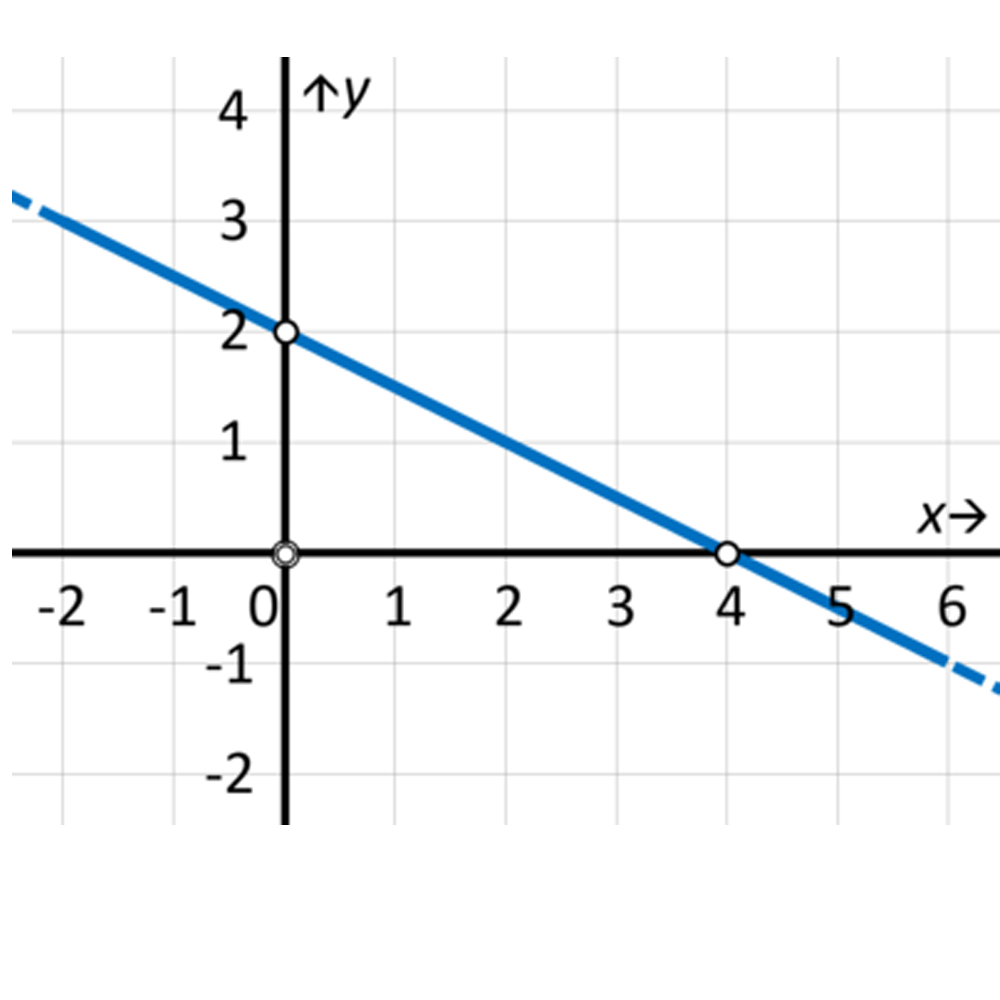
\includegraphics[scale=0.15]{imagenes/recta1.png} 
\caption{}
\label{etiqueta3}
\end{figure}

\item  ¿Cuál es el valor de la pendiente de la recta de la figura 4? \\
\begin{enumerate}
    \item $ m=2 $
    \item $ m=- 2 $  
    \item $ m= \frac{2}{3} $
    \item $ m= \frac{1}{2} $  
    \item $ m= -\ \frac{1}{2} $
    \end{enumerate}

\item  ¿Cuál es la ecuación de la recta de la figura 4? \\
\begin{enumerate}
    \item $ y= 4x + 2 $
    \item $ y=- 2 x + 2 $  
    \item $ y= \frac{1}{2} x \ -2 $
    \item $ y= \frac{1}{2} x \ +2$  
    \item $ y= -\ \frac{1}{2} x \ + 2 $
    \end{enumerate}
    
\item  Conociendo la ecuación de la recta ¿Qué valor tendrá $y$ con $x = 22$?  \\
\begin{enumerate}
    \item $ y= -9 $
    \item $ y= -11 $  
    \item $ y= -13 $
    \item $ y= -24 $  
    \item $ y= 13 $
    \end{enumerate}
    
\item  ¿Cuál de las siguientes ecuaciones podría reppresentar una recta paralela a la de la figura 4?  \\
\begin{enumerate}
    \item $ y= -3x +6 $
    \item $ y= - \frac{1}{2}x -3 $  
    \item $ y= - \frac{1}{4}x +3 $
    \item $ y= \frac{1}{2}x +3 $  
    \item $ y= 3x - 6 $
    \end{enumerate}
    
\item  ¿Cuál es la función inversa de la ecuación de la recta de la figura 4?  \\
\begin{enumerate}
    \item $ y= - \frac{1}{2}x -3 $
    \item $ y= 2x +4 $  
    \item $ y= 2x -4  $
    \item $ y= -2x + 4 $  
    \item $ y=- \frac{1}{4}x +3 $
    \end{enumerate}
    
 \end{enumerate} 
`\end{document}